\section{Results}
\label{sec:results}

\para{Overall performance.} \tabref{tab:main_results} reports clean, calibration, OOD, and adversarial metrics for all methods. The single model has the best clean accuracy (0.8828), ECE (0.0350), and NLL (0.3821). Random and orthogonal perturbation ensembles improve strong-attack robustness at PGD@8/255 (0.0050 and 0.0060) relative to the single model (0.0005), but both reduce clean accuracy by about 1.3 points.

\begin{table*}[t]
\centering
\resizebox{\textwidth}{!}{%
\begin{tabular}{@{}lccccccccc@{}}
\toprule
Method & Clean Acc & ECE $\downarrow$ & NLL $\downarrow$ & OOD AUROC & OOD AUPR & FPR95 $\downarrow$ & PGD@2/255 & PGD@4/255 & PGD@8/255 \\
\midrule
Single & {\bf 0.8828} & {\bf 0.0350} & {\bf 0.3821} & 0.8389 & 0.7680 & {\bf 0.7827} & {\bf 0.1375} & 0.0055 & 0.0005 \\
Random & 0.8699 & 0.0360 & 0.4138 & {\bf 0.8430} & {\bf 0.7705} & 0.7891 & 0.1195 & {\bf 0.0175} & 0.0050 \\
Orthogonal & 0.8702 & 0.0362 & 0.4129 & 0.8419 & 0.7663 & 0.7855 & 0.1190 & {\bf 0.0175} & {\bf 0.0060} \\
Adversarial & 0.8402 & 0.0894 & 0.5429 & 0.8228 & 0.7627 & 0.8468 & 0.1135 & 0.0045 & 0.0000 \\
\bottomrule
\end{tabular}%
}
\caption{Main evaluation metrics on CIFAR-10 (ID), SVHN (OOD), and PGD attacks. Best values are shown in bold for each metric. Higher is better except columns marked with $\downarrow$.}
\label{tab:main_results}
\end{table*}


\begin{figure}[t]
    \centering
    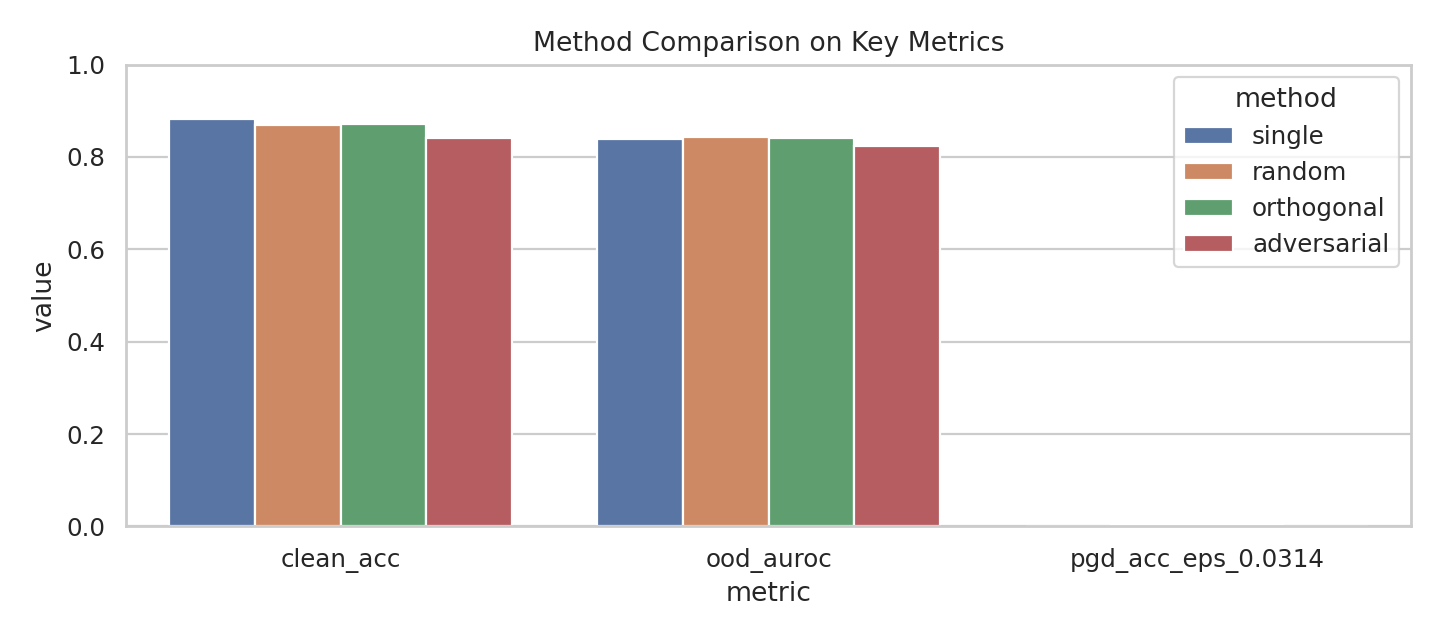
\includegraphics[width=0.95\linewidth]{figures/method_comparison_key_metrics.png}
    \caption{Comparison of key metrics across methods. Perturbation ensembles shift the clean--robustness trade-off: small gains under stronger attack come with clean-performance degradation.}
    \label{fig:key_metrics}
\end{figure}

\para{Statistical tests for primary hypotheses.} \tabref{tab:stats} shows bootstrap inference for predefined comparisons. Random perturbation ensembling improves PGD@8/255 over single by $+0.0045$ (95\% CI $[+0.0015,+0.0080]$, $p=0.004$), supporting a limited version of H1 at high attack strength. Orthogonal directions are not better than random ($p=0.599$), so H2 is not supported. Adversarial-direction perturbations are worse than random (difference $-0.0050$, $p<0.001$), refuting H3 in this setting.

\begin{table}[t]
\centering
\resizebox{\linewidth}{!}{%
\begin{tabular}{@{}lccc@{}}
\toprule
Comparison (difference) & Estimate & 95\% CI & $p$-value \\
\midrule
PGD@8/255: Random $-$ Single & +0.0045 & [+0.0015, +0.0080] & 0.004 \\
PGD@8/255: Orthogonal $-$ Random & +0.0010 & [-0.0020, +0.0040] & 0.599 \\
PGD@8/255: Adversarial $-$ Random & -0.0050 & [-0.0085, -0.0020] & $<0.001$ \\
Clean Acc: Random $-$ Single & -0.0129 & [-0.0172, -0.0086] & $<0.001$ \\
\bottomrule
\end{tabular}%
}
\caption{Bootstrap results for primary hypotheses. Differences are reported in absolute proportion units.}
\label{tab:stats}
\end{table}


\para{Diversity does not imply robustness.} \tabref{tab:diversity} shows that adversarial-direction perturbations produce much larger disagreement (0.2125) and much lower error correlation (0.4922) than random or orthogonal methods. However, this diversity increase does not improve robustness or OOD detection. Spearman analysis also fails to show positive association between disagreement and outcomes (disagreement vs OOD AUROC: $\rho=-0.20$, $p=0.8$; disagreement vs PGD@8/255: $\rho=-0.40$, $p=0.6$), so H4 is not supported.

\begin{table}[t]
\centering
\begin{tabular}{@{}lcc@{}}
\toprule
Method & Pairwise Disagreement & Pairwise Error Correlation \\
\midrule
Random & 0.00619 & 0.9788 \\
Orthogonal & 0.00544 & 0.9811 \\
Adversarial & {\bf 0.2125} & {\bf 0.4922} \\
\bottomrule
\end{tabular}
\caption{Diversity diagnostics among ensemble experts. Higher disagreement and lower error correlation indicate stronger diversity.}
\label{tab:diversity}
\end{table}


\begin{figure}[t]
    \centering
    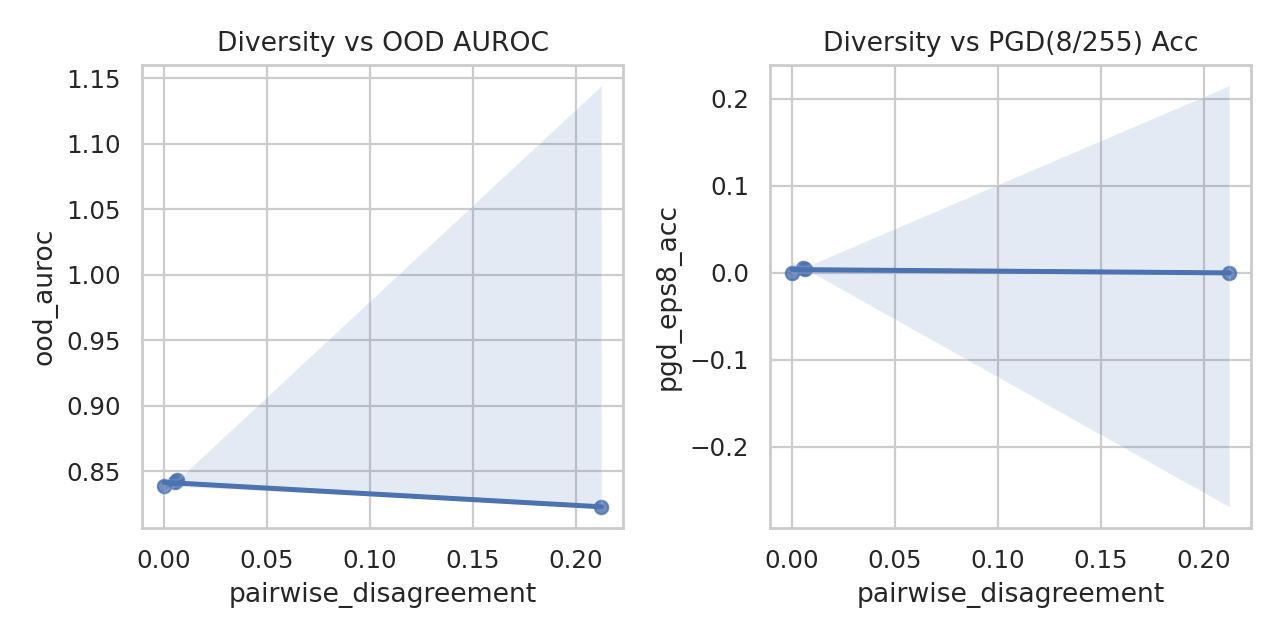
\includegraphics[width=0.95\linewidth]{figures/diversity_correlations.png}
    \caption{Correlation diagnostics between diversity and robustness/OOD metrics across methods. Larger disagreement does not map to better robustness in this experiment.}
    \label{fig:diversity_corr}
\end{figure}

\para{Runtime and reproducibility.} Full evaluation after checkpoint load takes 5.68 minutes on two RTX 3090 GPUs (24GB each), with fixed method seeds \{42, 101, 202, 303\}. This makes perturbation ensembling operationally lightweight, but the absolute robust accuracies remain very low ($<1\%$ at PGD@8/255) for all non-adversarially-trained methods.
